\chapter{Sistema, diseño y desarrollo}
\label{chap:sistemadesarrollado}

\section{Estructura general del sistema}

El sistema desarrollado se ha basado en \textit{Docker} para evitar problemas de configuración y portabilidad, es decir, podrá ser desplegado en cualquier sistema que soporte esta tecnología. La estructura está basada en varias capas, todas ellas sobre el sistema anfitrión que elijamos, pudiendo adaptarse incluso a un servidor. En la figura   \ref{fig:DiagramaDelSistema} se puede apreciar la distribución de las capas mencionadas. 

\begin{itemize}
\item La primera capa de esta estructura es el propio sistema anfitrión que, normalmente, será el equipo de utilice el usuario regularmente. Su única función es la de servir de base para la ejecución de la imagen {\itshape{Docker}}.
\item Inmediatamente por encima del sistema anfitrión se encuentra la imagen {\itshape{Docker}}, encargada de facilitar la configuración y las dependencias necesarias para la ejecución de {\itshape{Galaxy}}.
\item La imagen {\itshape{Docker}} incluye el despliegue de {\itshape{Galaxy}} sobre el puerto 8080. Por lo que podemos considerar como otra capa del sistema a la propia ejecución de {\itshape{Galaxy}}.
\item El punto principal del trabajo se encuentra en el apartado de workflows dentro de {\itshape{Galaxy}}. En él se localiza la secuencia de herramientas que conforma el núcleo del proyecto.
\item Exteriormente a {\itshape{Galaxy}} y {\itshape{Docker}}, se han desarrollado dos herramientas que interactúan con el workflow. La primera es un script {\itshape{Python}} que se encarga de toda la configuración y ejecución del workflow, para facilitar su utilización a usuarios no experimentados en informática. La segunda herramienta se encarga de tratar los datos obtenidos de la ejecución para generar un formato más fácil de comprender y manipular por el usuario.
\end{itemize}

\begin{figure}
    \begin{center}
      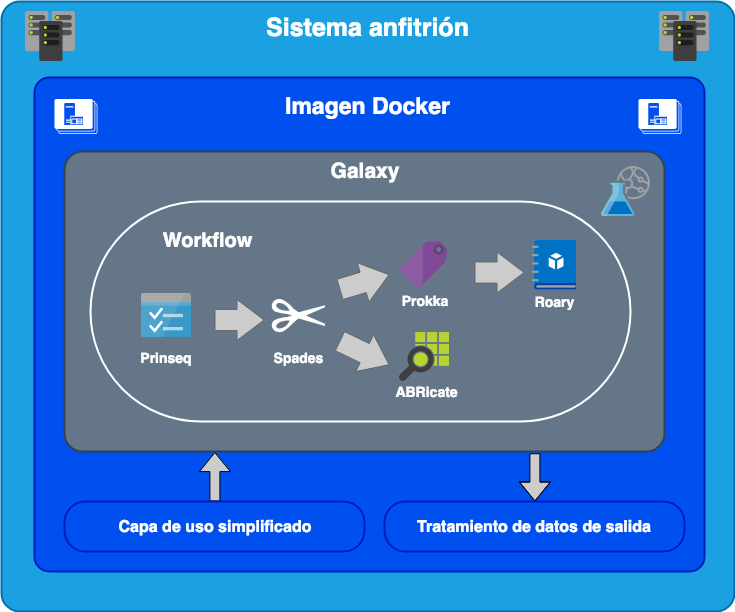
\includegraphics[scale=0.5]{images/DiagramaDelSistema.png}
      \caption{Estructura del sistema}
      \label{fig:DiagramaDelSistema}
    \end{center}
\end{figure}
\section{Desarrollo y configuración de \itshape{Docker}}
La imagen \textit{Docker} utilizada está basada, con algunas modificaciones, en la desarrollada por Sergio Chico en su Trabajo de Fin de Máster \cite{Chico2018}. La cual, a su vez, hereda de una imagen \textit{Docker Galaxy} estable desarrollada por Björn A. Grüning \cite{GalaxyDocker}.

Utilizando como punto de partida la imagen de Sergio Chico, se han realizado una serie de adaptaciones para adecuarla al uso de nuestro workflow. La primera modificación realizada fue la instalación de las nuevas herramientas necesarias que no estaban disponibles en ese momento. Al conjunto de herramientas iniciales se añadieron \textit{Prinseq}, \textit{Spades}, \textit{Roary}, \textit{ABRicate} y \textit{Prokka}. Además, en las opciones de instalación de herramientas de \textit{Galaxy} solo estaba disponible para la versión previa de \textit{Roary} que producía, por algún tipo de bug, ficheros de salida vacíos. Por lo tanto, se creó una nueva herramienta a partir de la original con la nueva versión disponible para escritorio de \textit{Roary}.

Una vez realizadas estas adaptaciones a la imagen, se ha dejado disponible en \textit{Dockerhub} bajo el nombre \textit{jbarberoaparicio/workflowmanager}\footnote{https://hub.docker.com/r/jbarberoaparicio/workflowmanager}. 

Además de esto, se han desarrollado varios scripts simples para facilitar el uso de \textit{Docker}. El primero de ellos se encarga del montaje completo de la imagen a partir del \textit{Dockerfile}, en caso de que quisieran realizarse modificaciones en un futuro. El segundo se encarga del arranque de la imagen desplegándola a través de \textit{Docker}. El tercero se desarrolló para resolver un bug en \textit{OSX} por el cual los ficheros eliminados dentro de la imagen no se eliminaban correctamente. Esto provocaba que un fichero tipo \textit{log} ocupase todo el espacio disponible en el disco. El script se encarga de eliminar esta información sin borrar las imágenes existentes.


\section{Desarrollo y configuración del workflow en \itshape{Galaxy}}
A lo largo del workflow, se realizarán varios análisis diferenciados de las secuencias. En algunos casos estos análisis servirán  únicamente de entrada para el siguiente paso y en otros aportarán por sí mismos parte de la información deseada. 
Cabe destacar que se ha definido la entrada del workflow como un formato de dos colecciones, una para cada dirección de las lecturas de las secuencias. 

\subsection{\itshape{Trimmomatic}}
Como se ha explicado en el capítulo \ref{chap:estadodelarte}, la secuenciación con la tecnología \textit{Illumina} implica la utilización de primers y adaptadores que deben ser eliminados para un correcto procesamiento posterior. Para ello, se ha decidido utilizar la herramienta \textit{Trimmomatic}~\cite{Bolger2014}, que incluye diferentes protocolos orientados a diferentes tecnologías de \textit{Illumina} como \textit{MiSeq} o \textit{HiSeq}.

\textit{Trimmomatic} se encargará de recibir los dos ficheros \textit{fastq} iniciales emparejados de cada cepa y les aplicará el protocolo de filtrado adecuado. En este caso se ha utilizado \textit{Nextera}, dado que la secuenciación se llevó a cabo con un equipo \textit{HiSeq}. Una vez eliminadas las secuencias de primers y adaptadores, los nuevos ficheros \textit{fastq} se enviarán a \textit{Prinseq} para realizar a las secuencias un control de calidad.

\subsection{\itshape{Prinseq}}
Con el objetivo de realizar un filtrado de calidad de las secuencias, se ha utilizado \textit{Prinseq}~\cite{schmieder_prinseq}. Esta herramienta, desarrollada en \textit{Perl}, ofrece la posibilidad de generar un informe en el cual se indican diferentes estadísticas sobre la calidad de cierta secuencia. Además, utiliza esa información para realizar el filtrado que le indiquemos, pudiendo ser en función de la longitud de las lecturas o de su calidad.

Como formato de entrada, introduciremos en \textit{Prinseq} un fichero \textit{fastq}. En esta situación, proveniente de los resultados de \textit{Trimmomatic}. Como salida, obtendremos otro fichero \textit{fastq} en el que se habrán eliminado todos los fragmentos que no hayan cumplido las condiciones que se hayan fijado en los parámetros de ejecución. Para nuestro caso, se han eliminado las secuencias de longitud menor que 50 y de índice de calidad menor de 15. El resto de parámetros se han mantenido por defecto a excepción de la indicación de que se trata de una secuencia <<paired-end>>, necesaria para la ejecución de la manera en la que deseamos llevarla a cabo.

\textit{Prinseq} ha sido una de las herramientas que menos complicaciones ha presentado a lo largo del proyecto, devolviendo errores comprensibles cuando las ejecuciones no eran correctas y ofreciendo toda la información necesaria para resolverlo. A pesar de ello, la versión de \textit{Prinseq} disponible en \textit{Galaxy} tiene la desventaja de no generar el informe con todas las estadísticas resultantes que sí genera su versión web.

\subsection{\itshape{SPAdes}}
\textit{SPAdes}~\cite{Nurk2013} ha sido la utilidad seleccionada para la fase de ensamblado. Se trata de un conjunto de herramientas que facilitan un modo de recoger todas las lecturas validadas en el proceso de filtrado y encadenarlas de la manera en la que corresponden en la secuencia. Fue desarrollado enfocándose a genomas pequeños, como bacterias y hongos. Por lo tanto, se adapta bien al caso de uso que estamos tratando.

Para su ejecución, se debe indicar a \textit{SPAdes} la estructura que estamos siguiendo en el workflow, introduciendo ficheros separados en los dos sentidos de lectura de las secuencias en forma de colecciones. Estos ficheros provendrán de la salida de la ejecución de \textit{Prinseq}, tras realizar el filtrado de calidad. El resto de parámetros de la ejecución, a excepción de la longitud de los k-mer, establecida a 77, se han mantenido por defecto. También se le ha indicado que las bibliotecas a utilizar sean <<paired-end>>.

Dado el gran tamaño de las lecturas de los casos en los que el workflow ha sido probado, \textit{SPAdes} ha resultado problemático por tener que almacenar en RAM todas las lecturas al mismo tiempo. Esto ha implicado que, para las muestras de prueba, se haya requerido de 16 GB de memoria RAM para poder ejecutarlo. Además, los mensajes de error de la versión \textit{Galaxy} de \textit{SPAdes} no dan demasiada información en muchos casos. En algunos otros, relacionados con la capacidad de memoria, no se producía ningún mensaje de error, sino que se daba por correcta la ejecución a pesar de que los ficheros retornados estaban vacíos. A pesar de estos problemas de desarrollo, \textit{SPAdes} ha terminado cumpliendo su función correctamente tras identificar los errores del proceso. 

\subsection{\itshape{ABRicate}}
Uno de los principales intereses al comenzar el proyecto era el análisis de resistencia a antibióticos de las cepas. \textit{ABRicate}~\cite{seemann_:mag_right:_2019} es una herramienta desarrollada en \textit{Perl} que permite la localización de genes vinculados a resistencia a antibióticos o relacionados con virus realizando un cribado masivo de los contigs introducidos. Para ello utiliza las bases de datos de \textit{Resfinder}~\cite{Resfinder}, \textit{CARD}~\cite{CARD}, \textit{ARG-ANNOT}~\cite{Gupta212}, \textit{NCBI} \textit{BARRGD}, \textit{EcOH}, \textit{PlasmidFinder}~\cite{Carattoli3895}, \textit{Ecoli\_VF} y \textit{VFDB}~\cite{VFDB}. En nuestro caso, ese input serán los contigs obtenidos por \textit{SPAdes} para cada una de las secuencias. Esta herramienta forma uno de los finales del workflow, es decir, su salida no sirve como entrada a ninguna otra herramienta sino que los datos que se obtienen de ella tienen su utilidad propia.

La configuración de \textit{ABRicate} es muy sencilla y ofrece pocas posibilidades de variación, por lo que no ha sido necesario modificar ningún parámetro de la herramienta. La ejecución por defecto no ha presentado problemas.

Una de las limitaciones de \textit{ABRicate} es que no admite lecturas tipo \textit{fastq}, solamente contigs. En nuestro caso los contigs provienen de la salida de \textit{SPAdes}, por lo que es una herramienta adecuada.

\subsection{\itshape{Prokka}}
Para la fase de anotación se ha decidido utilizar \textit{Prokka}~\cite{Seemann2014}, una herramienta desarrollada en \textit{Perl} destinada específicamente a genomas procariotas y que destaca por su rapidez. El proceso de anotación de \textit{Prokka} se divide en dos fases. En la primera, se utiliza \textit{Prodigal} para la identificación de regiones codificadoras de proteínas. En la segunda, se compara con varias bases de datos para reconocer, por similitud, cuál es la proteína de la que se trata.

La configuración de \textit{Prokka} en \textit{Galaxy} no ha resultado complicada a pesar de que los parámetros son numerosos. El único problema encontrado en la configuración ha sido a raíz del formato \textit{gff3}. A pesar de que se indique que los ficheros de salida siguen esa estructura, realmente no es así, sino que internamente son formato \textit{gff}. Para solucionar este inconveniente se ha añadido una fase nueva en el workflow, en la que una herramienta simple de concatenación une la salida \textit{gff} con la propia secuencia del genoma.

\subsection{\itshape{Roary}}
Uno de los objetivos principales del proyecto era la realización de un análisis pangenómico. Utilizando como entrada las anotaciones provenientes de \textit{Prokka} de todas las muestras, \textit{Roary}~\cite{Page2015} se encarga de calcular el pangenoma. Ha resultado ser una herramienta realmente rápida, con la que en unos minutos se obtienen los resultados.

\textit{Roary} está desarrollado para recibir ficheros gff3 desde \textit{Prokka}, por lo que no debería haber problemas de compatibilidad (una vez solucionado el error de formato comentado en el punto anterior). El problema con la configuración de \textit{Roary} dentro del workflow es que, si se instala desde el repositorio oficial en el \textit{Tool Shed} de \textit{Galaxy}, no se obtiene ningún tipo de contenido en los ficheros de salida. Estudiando este problema, se llegó a la conclusión de que se podría deber a que la versión disponible en este repositorio no es la versión final publicada para escritorio. Por lo tanto, se creó una herramienta \textit{Galaxy} nueva utilizando la versión standalone de \textit{Roary}. Una vez disponible esta herramienta en \textit{Galaxy} y manteniendo la configuración establecida para la versión anterior, los ficheros fueron obtenidos correctamente.

\textit{Roary} recibe todos los ficheros tratados por el workflow (a excepción de la salida independiente de \textit{ABRicate}) y sirve como herramienta final. La clasificación de cada cepa según su mejor coincidencia para cada gen con el pangenoma creado por \textit{Roary} no son enviados a ninguna otra herramienta dentro de \textit{Galaxy} y finalizan el workflow.


\section{Desarrollo de la capa externa con \itshape{Python}}
A pesar de que el workflow completo ha sido desarrollado dentro de \textit{Galaxy}, se han añadido algunas funcionalidades extra utilizando \textit{Python}.

\subsection{Capa de uso simplificado}
Dado que el equipo al que está destinada la herramienta no pertenece al campo de la informática, se solicitó una herramienta que fuese sencilla de utilizar. Por ello, se ha creado un script que realiza todos los pasos necesarios para ejecutar el workflow simplemente con ejecutarlo, sin ser necesario ningún tipo de configuración. En caso de que el usuario tuviese conocimientos técnicos, seguirá teniendo la posibilidad de utilizar la herramienta sin este script.

Para ello, se ha utilizado la API de \textit{Galaxy}, parte de la librería \textit{BioBlend}\footnote{\url{https://bioblend.readthedocs.io/en/latest/}}. Esta API nos permite controlar todos los aspectos de una instancia \textit{Galaxy} desde código \textit{Python}.

Desde el script se crea una sesión en la instancia de \textit{Galaxy} a partir de la cual se realizan todas las tareas. Una vez conectado, el script carga el archivo que almacena el workflow que va a ejecutar. Después, para mantener los datos aislados e identificados, crea historiales nuevos para los ficheros de entrada y los de salida con un nombre único a partir de la fecha y hora de creación. A continuación carga los datos brutos de inicio, lo que, dependiendo de su tamaño, puede llevar unos minutos. Para que el workflow funcione correctamente, necesita recibir los datos en forma de colección, por lo que el script se encarga de crear una para cada conjunto de datos, es decir, lecturas en un sentido y en el inverso. El paso siguiente, la ejecución del workflow, es el fundamental y el más costoso en tiempo. Para controlar el estado de la tarea en cada momento, se va realizando un control cada pocos segundos que comprueba si las tareas siguen en proceso. Una vez finalizado, los datos de salida se mantienen en un historial propio, pero para poder utilizarlos fuera de \textit{Galaxy}, el script se encarga de almacenarlos en el disco local del equipo en una carpeta con el nombre del historial.

\subsection{Agrupación de resultados}
Para facilitar el acceso a los resultados de todas las herramientas, se ha planteado la creación de un solo fichero que pueda abrirse con \textit{Excel}, herramienta que resulta familiar al grupo que utilizará el workflow. Para ello, desde un script de \textit{Python} se genera un solo fichero en el que cada hoja contiene los resultados de uno de los pasos del workflow.